\documentclass[a0,portrait]{a0poster}

\columnsep=100pt % This is the amount of white space between the columns in the poster
\columnseprule=3pt % This is the thickness of the black line between the columns in the poster


% Пакеты для математических символов:
\usepackage{amsmath} % Американское математическое сообщество
\usepackage{amssymb} % Расширенные символы
\usepackage{amsthm}  % Окружения для теорем, определений и т.д.
\usepackage{physics} % Основные физические символы
\usepackage{tikz-feynhand} % Для создания фейнмановских диаграмм

% Пакеты для шрифтов:
\usepackage[utf8]{inputenc} % Кодировка символов
\usepackage[T1, T2A]{fontenc} % Кодировка шрифта
\usepackage[english, russian]{babel} % Языки (английский и русский)

% Цвета:

% Оформление ссылок:
\usepackage{hyperref}
\hypersetup{
    colorlinks=true,
    linkcolor=black,
    filecolor=magenta,      
    urlcolor=cyan,
    pdftitle={Overleaf Example},
    pdfpagemode=FullScreen,
    }
    
\usepackage{xcolor} %Позволяет перекрасить все страници
\definecolor{SteelBlue}{RGB}{100,149,237} % Цвет для рамок

% Оформление текста и полей:

\usepackage[framemethod=TikZ]{mdframed} % Красивые рамки
\usepackage{graphicx} % Работа с изображениями
\usepackage{multicol} % Разделение текста на несколько колонок
\usepackage{wrapfig} % вставка картинок и таблиц, обтекаемых текстом.
\usepackage{titlesec} % Управление заголовками секций
\usepackage{array}    % Расширенные таблицы
\usepackage{anyfontsize}
\usepackage{subcaption} % возможность вставлять картинки в строчку
\usepackage{cancel} % значки для сокращения дробей, упрощения, стремления.
\usepackage{multirow} % Многострочные формулы
\usepackage{caption} % Названия без нумерации
\usepackage[backend=biber, style=gost-numeric]{biblatex} % Литература по госту
\usepackage{hyperref} % Ссылки как внешние так и внутренние
\hypersetup{
    colorlinks=true,
    linkcolor=black,
    filecolor=magenta,      
    urlcolor=cyan,
    pdftitle={Overleaf Example},
    pdfpagemode=FullScreen,
    }

% Оформление рамок:
\mdfdefinestyle{MyFrame}{%
    linecolor=SteelBlue,
    outerlinewidth=2pt,
    roundcorner=50pt,
    innertopmargin=\baselineskip,
    innerbottommargin=\baselineskip,
    innerrightmargin=20pt,
    innerleftmargin=20pt,
    backgroundcolor=white!50!white
}

% Пользовательские команды:
\newcommand{\inrad}[1]{\left( #1 \right)}
\newcommand{\inner}[1]{\left( #1 \right)}
\newcommand{\infig}[1]{\left\{ #1 \right\}}
\newcommand{\insqr}[1]{\left[ #1 \right]}
\newcommand{\ave}[1]{\left\langle #1 \right\rangle}

% Пользовательские символы:
\renewcommand{\geq}{\geqslant}
\renewcommand{\leq}{\leqslant}
\renewcommand{\phi}{\varphi}
\renewcommand{\epsilon}{\varepsilon}

% Пользовательские функции:
\newcommand{\rot}{\text{rot}}
\renewcommand{\div}{\text{div}}
\renewcommand{\grad}{\text{grad}}
\newcommand{\llp}[1]{\lambda_{\Lambda_{#1}}}



\newcommand\tab[1][0.51cm]{\hspace*{#1}}




% Начало документа:
\begin{document}

\begin{mdframed}[style=MyFrame]
\vspace{0.5cm} 
    % Заголовок плаката:
    \begin{minipage}[b]{0.1\linewidth}
        \centering
        
\includegraphics[width=1\linewidth]{img/KEK_logo.jpg}
    \end{minipage}
    \begin{minipage}[b]{0.75\linewidth}
        \centering
        {\Huge{\textbf{Измерение формфакторов полулептонных распадов}} $\Lambda_c$} \\ \vspace{1em}
        {\huge \textbf{\underline{Карибджанов М. Р.}, Пахлов П. Н., Ясавеев М. И.}} \\[0.5em]
    \end{minipage}
    \begin{minipage}[b]{0.1\linewidth}
        \centering
        
\includegraphics[width=1\linewidth]{img/logo_hse_cmyk.jpg}
    \end{minipage}
\vspace{0.5cm}

\begin{multicols}{2}

% Разделы текста:
\section{Мотивация}

\tab $\Lambda_c$, будучи самым лёгким из очарованных барионов, распадается 
исключительно посредством слабого взаимодействия, благодаря чему является 
эталоном исследования слабого взаимодейтвия среди очарованных барионов, 
при этом на данный момент существует одно исследование эксперимента CLEO по 
измерению формфакторов $\Lambda_c \to \Lambda e \nu_e$. Так же существует 
несколько численных расчетов по измерению формфакторов в различных приближениях.

\section{Выражение формфакторов}

\tab Используя выражение спиральных амплитуд в системе отсчета $\Lambda_c$ 
через матричные элементы тока слабого перехода и поляризации $W$-бозона, получим:

\begin{multicols}{2}
    \begin{equation*}
    H^{V}_{t\frac{1}{2}} = \frac{\sqrt{Q_+}}{\sqrt{q^2}} \inrad{ \mathfrak F_1^V \inrad{ M_{\Lambda_c} - M_{\Lambda} } + \mathfrak F_3^V \frac{q^2}{M_{\Lambda_c}} },
    \end{equation*}
    \begin{equation*}
    H^{V}_{1\frac{1}{2}} = \sqrt{2Q_-} \inrad{ - \mathfrak F_1^V - \mathfrak F_2^V \frac{M_{\Lambda_c} + M_{\Lambda}}{M_{\Lambda_c}} },
    \end{equation*}
    \begin{equation*}
    H^{V}_{0\frac{1}{2}} = \frac{\sqrt{Q_-}}{\sqrt{q^2}} \inrad{ \mathfrak F_1^V \inrad{ M_{\Lambda_c} + M_{\Lambda} } + \mathfrak F_2^V \frac{q^2}{M_{\Lambda_c}} },
    \end{equation*}
    \begin{equation*}
    H^{A}_{t\frac{1}{2}} = \frac{\sqrt{Q_-}}{\sqrt{q^2}} \inrad{ - \mathfrak F_1^A \inrad{ M_{\Lambda_c} + M_{\Lambda} } + \mathfrak F_3^A \frac{q^2}{M_{\Lambda_c}} },
    \end{equation*}
    \begin{equation*}
    H^{A}_{1\frac{1}{2}} = \sqrt{2Q_+} \inrad{ \mathfrak F_1^A - \mathfrak F_2^A \frac{M_{\Lambda_c} - M_{\Lambda}}{M_{\Lambda_c}} },
    \end{equation*}
    \begin{equation*}
    H^{A}_{0\frac{1}{2}} = \frac{\sqrt{Q_+}}{\sqrt{q^2}} \inrad{ - \mathfrak F_1^A \inrad{ M_{\Lambda_c} - M_{\Lambda} } + \mathfrak F_2^A \frac{q^2}{M_{\Lambda_c}} },
    \end{equation*}
\end{multicols}

Где $q^\mu$ --- 4-импульс $W$-бозона, $M_x$ --- масса частици $x$, $Q_\pm = \inner{M_{\Lambda_c} \pm M_{\Lambda}}^2 - q^2$, 
$\mathfrak F_\mu^{A, V}$ --- формфакторы, $H_{\lambda_W \lambda_\Lambda}^{A, V}$ --- спиральная амплитуда, $A$ --- аксиальная компонента, $V$ --- векторная, $\lambda_x$ --- спиральность частици $x$, $t$ --- синглетное сотояние $W$-бозона. 
Решение данной системы уранений позволяет свети задачу к вычислению спральных амплитуд.


\section{Метод измерения спиральных амплитуд}

\tab С помощью формализма спиральных амплитуд можно описать процесс 
$\Lambda_c \to \Lambda l \nu_l$ и получить его угловое распределение.  

\begin{multline*}
    \frac{d\Gamma}{dq^2 d\cos\theta_l d\cos\theta_p d\cos\theta_d d\phi_l d\phi_p d\chi} \propto f^{\Lambda_l \nu_l}_{\text{sig}}\inner{\theta_\Lambda, \theta_l, \theta_p, \phi_\Lambda, \phi_l, \phi_p; P_L, H^{V, A}_{\lambda_\Lambda \lambda_W}} = q^2 \sqrt{Q_+ Q_-}  \times \\
    \left\{ H_{1\frac{1}{2}}^2 \inrad{1 - P_L \cos\theta_\Lambda} \inrad{1 + \alpha_\Lambda \cos\theta_p} \inrad{1 \pm \cos\theta_l}^2
    + H_{-1\frac{1}{2}}^2 \inrad{1 + P_L \cos\theta_\Lambda} \inrad{1 - \alpha_\Lambda \cos\theta_p} \inrad{1 \mp \cos\theta_l}^2 + \right. \\
    + 2 \sin^2\theta_l \left[ H_{0\frac{1}{2}}^2 \inrad{1 + P_L \cos\theta_\Lambda} \inrad{1 + \alpha_\Lambda \cos\theta_p} + H_{0\frac{1}{2}}^2 \inrad{1 - P_L \cos\theta_\Lambda} \inrad{1 - \alpha_\Lambda \cos\theta_p} \right] - \\
    - 2\sqrt{2} \alpha_\Lambda \sin\theta_p \sin\theta_l \cos\chi \left[ H_{1\frac{1}{2}} H_{0\frac{1}{2}} \inrad{1 - P_L \cos\theta_\Lambda} \inrad{1 \mp \cos\theta_l} + H_{-1\frac{1}{2}} H_{0\frac{1}{2}} \inrad{1 + P_L \cos\theta_\Lambda} \inrad{1 \pm \cos\theta_l} \right] -\\
    - 2\alpha_\Lambda P_L \sin\theta_\Lambda \sin\theta_p \sin^2\theta_l \left[ 2H_{0\frac{1}{2}} H_{0\frac{1}{2}} \cos\varphi + H_{1\frac{1}{2}} H_{-1\frac{1}{2}} \cos(\varphi + 2\chi) \right] +\\
    + 2\sqrt{2} P_L \sin\theta_\Lambda \sin\theta_l \cos(\varphi + \chi) \left[ H_{1\frac{1}{2}} H_{0\frac{1}{2}} \inrad{\mp 1 + \alpha_\Lambda \cos\theta_p} \inrad{1 \pm \cos\theta_l} \right] \\
    \left.+ H_{-1\frac{1}{2}} H_{0\frac{1}{2}} \inrad{\mp 1 - \alpha_\Lambda \cos\theta_p} \inrad{1 \mp \cos\theta_l} \right\}
\end{multline*}
Где $\pm$ сответствует: плюс --- сотоянию $\Lambda_c^+$, минус --- сотоянию $\Lambda_c^-$.

\begin{wrapfigure}[15]{l}{13cm}
    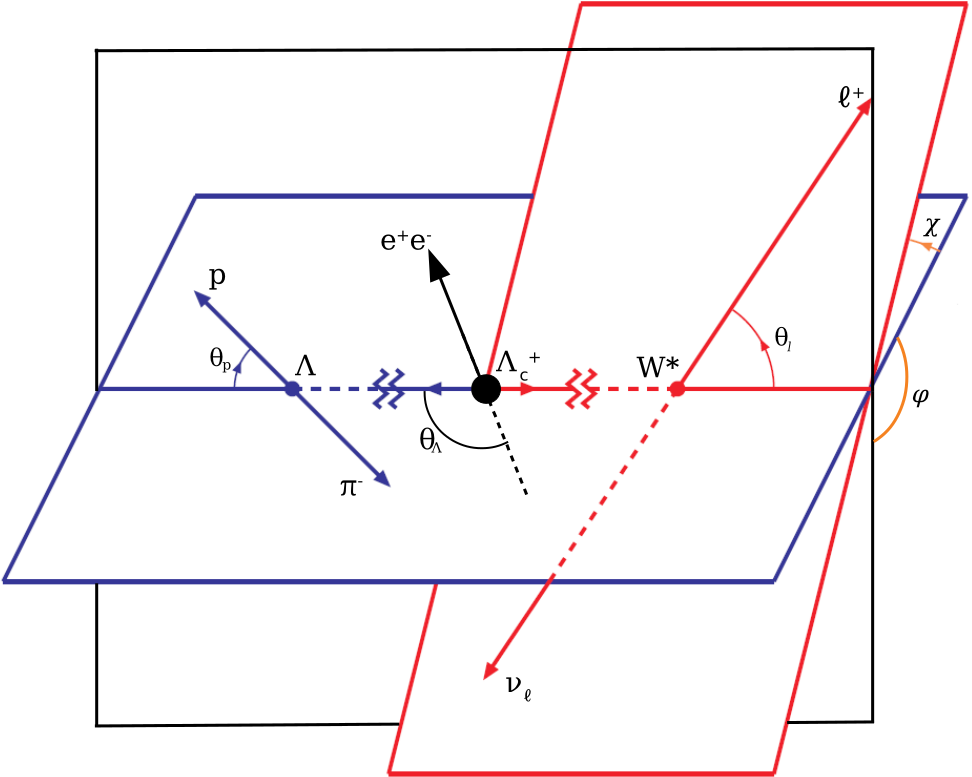
\includegraphics[width=15cm]{img/lc_l_l_nu_def.png}%
    \captionsetup{justification=centering,margin=2cm}
    \caption{Кинематика распада $\Lambda_c \to \Lambda l \nu_l$}
    \label{kin:lepton:img}
\end{wrapfigure}



Где переменные (рис. \ref{kin:lepton:img}): в системе отсчета $\Lambda_c$ с осью $z$ вдоль импульса $e^+ e^-$, 
$\theta_\Lambda, \ \phi_\Lambda$ --- полярные углы $p_\Lambda$;  
в системе отсчета $W$-бозона с осью $z$ вдоль импульса $\Lambda_c$, $\theta_l, \phi_l$ --- углы $p_l$; 
так же введены следующие сокращения $\phi = \phi_p - \phi_\Lambda , \chi = \pi - \phi_l - \phi_p$.
$\theta_p, \ \phi_p$ --- углы $p_p$. 
И измеряемые параметры: $P_L$ --- продольная поляризация $\Lambda$, 
$H^{V, A}_{\lambda_\Lambda \lambda_W}$ --- спиральные амплитуды.

\tab Для уменьшения количества фитируемых параметров можно рассмотреть случай перехода 
$W^\pm$-бозона в $\pi^\pm$, в таком случае угловое распределение будет описываться:

\begin{multline*}
    \cfrac{dW_{\llp{c}}}{d\cos{\theta_p}d\cos{\theta_p}d\phi_{\llp{c}}\phi_{\llp{p}}} \propto f_{sig}^{\Lambda\pi} 
    =
    1 + \alpha_{\Lambda}\alpha_{\Lambda_c} \cos \theta_p + \\
    \hspace{-20mm}
    + P_L\insqr{\cos\inner{\alpha_{\Lambda} + \alpha_{\Lambda_c} \cos{\theta_p}} - 
    \alpha_{\Lambda}\sqrt{1 - \alpha_{\Lambda_c}^2}\cos\inner{\delta + \Delta}\cos\theta_p \cos \theta_\Lambda}
    \label{spin:Lam:pdf}
\end{multline*}

Где обозначения переменных сохранены. Новые переменные (рис. \ref{kin:pi:img}), $\delta$ --- фаза между спиральными амплитудами 
$W$-бозона и является фитируемым параметром, и $\Delta$ --- угол между плоскостью $p_{e^+ e^-}, \ p_{\Lambda_c}$ и $p_p, \ p_\pi$.

\begin{minipage}{\columnwidth}
    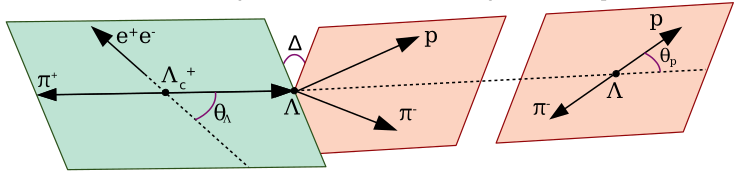
\includegraphics[width=0.9\columnwidth]{img/lpi_def.png}   
    \captionsetup{justification=centering,margin=2cm}
    \captionof{figure}{Кинематика распада $\Lambda_c \to \Lambda \pi$}
    \label{kin:pi:img}
\end{minipage}

\section{Тагирование}

\tab Для востановления $\nu$ в полулептонном канале, улучшения разрешения в канале $\Lambda \pi$, 
использовалась технология тагирования, для чего рассматривались 
события $e^- e^+ \to \Lambda_c X_c$, где $X^+_c = D^0 p; D^+ p \pi^-; D^{*0} p; D^{*+} p \pi^-$. 
Инклюзивный отбор событий происходил по следующим критериям:

\begin{multicols}{2}
    \begin{itemize}
        \item $\mathfrak L \inner{K/\pi, K/p} > \infig{0.6, 0.6}$
        \item $\mathfrak L \inner{p/\pi, p/K} > \infig{0.6, 0.4}$
        \item $goodBelleKshort = 1$
        \item $E_{\gamma} > 50 MeV$
        \item $\abs{M_{K_S} - M^{PDG}_{K_S}} < 15 MeV$
        \item $\abs{M_{D} - M_{D}^{PDG}} < 15 MeV$
        \item $\abs{M_{D^*} - M_{D^*}^{PDG}} < 2 MeV$
    \end{itemize}
    Для всех заряженных треков 
    \begin{itemize}
        \item $dz < 2 cm; dr < 0.5 cm$;
        \item $\abs{M_{\pi^0} - M^{PDG}_{\pi^0}} < 15 MeV$.
    \end{itemize}
\end{multicols}

Где $goodBelleKshort$ --- кат принятый и оптимизированный в $Belle$ для $K$-мезонов. 

\vspace{0.5cm}

\tab По итогу отбора было получено (рис. \ref{dist:rec:M})

\begin{minipage}{\columnwidth}
    \centering
    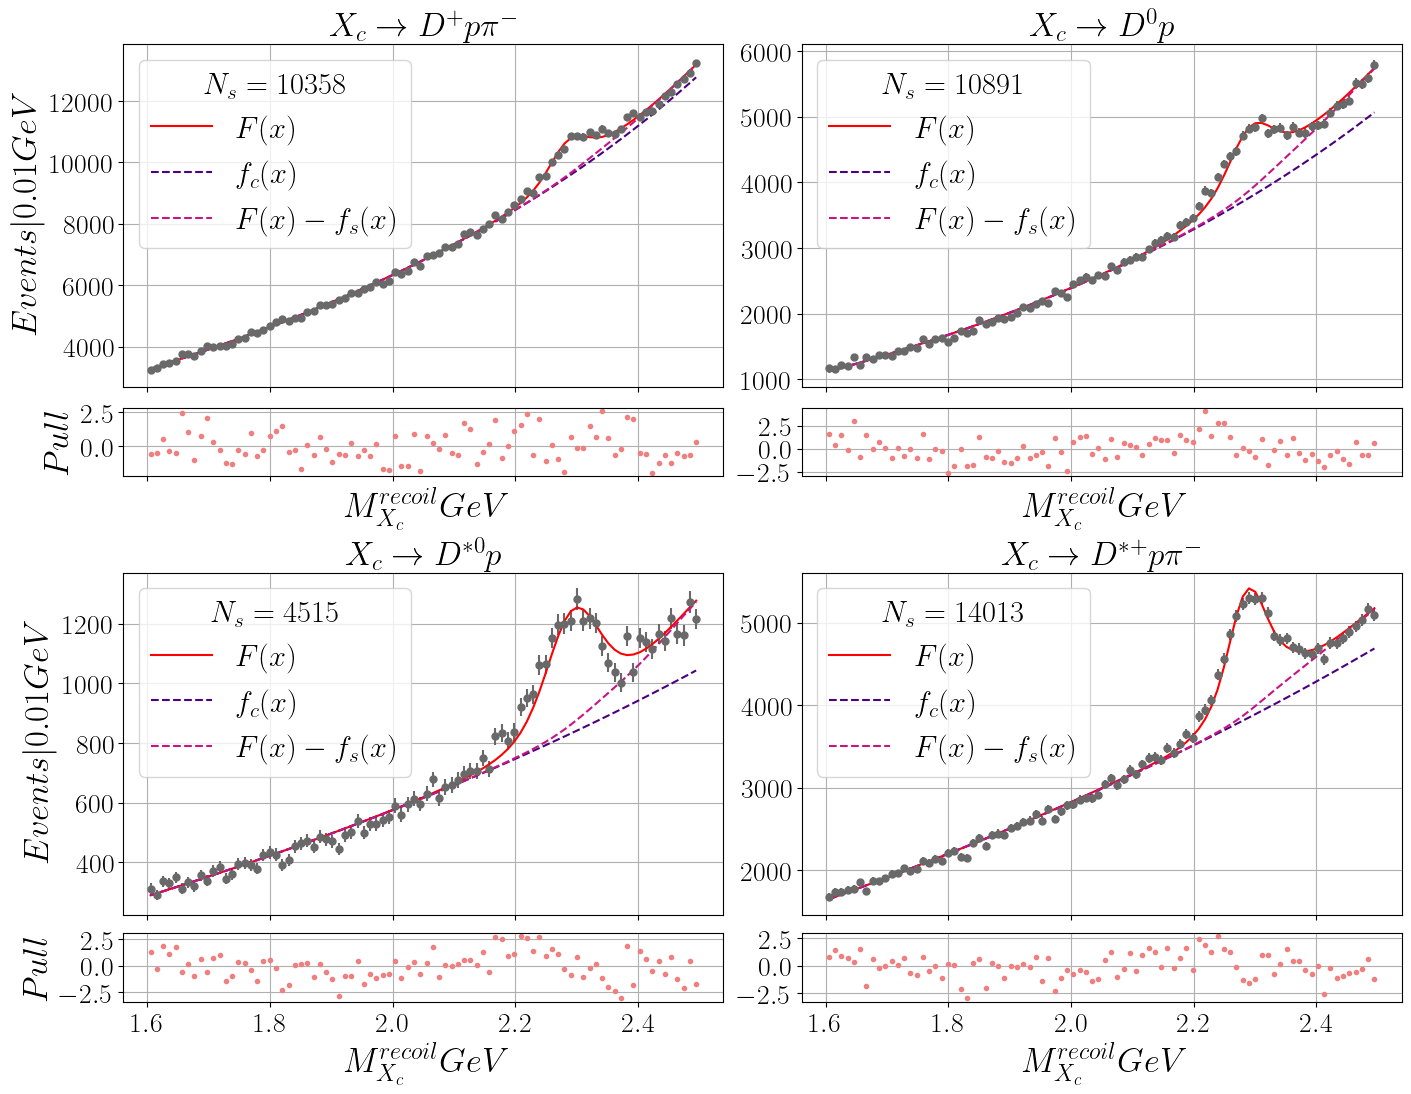
\includegraphics[width=0.9\columnwidth]{img/inc_res.png}
    \centering
    \captionsetup{justification=centering,margin=2cm}
    \captionof{figure}{Количество сигнальных событий в каналах $X_c$.\\
    $N_s$ --- предполагаемое кол-во затагированных $\Lambda_c$}
    \label{dist:rec:M}
\end{minipage}

\vspace{0.5cm}


Подгонка данных производилась функцией:

\begin{equation*}
    F(x) = f_s(x) + f_c(x) + f_{bg}(x) 
\end{equation*}

Где $f_s(x)$ --- сигнальная функция гауссовой формы; $f_c(x)$ --- функция комбинаторного фона экспоненциальной формы; 
$f_{bg}(x)$ --- функция потерь растет корневым образом начиная с массы $\Lambda_c$.

%\begin{tabular}{||c|c|c||}
%    \hline
%    $X_c$ & $N_{sig}$ & $\sigma \insqr{MeV}$ \\ \hline 
%    $ \ D^0 p \ $ & $\ 10124\pm1402 \ $ & $ \ 66.7 \ $ \\ \hline
%    $ \ D^+ p \pi^- \ $ & $\ 9845\pm1471 \ $ & $ \ 54.4 \ $ \\ \hline
%    $ \ D^{*0}p \ $ & $\ 4153+377 \ $ & $ \ 62.2 \ $ \\ \hline
%    $ \ D^{*+} p \pi^- \ $ & $\ 13458\pm1115 \ $ & $ \ 51.1 \ $ \\ \hline 
%\end{tabular}

\section{Эксклюзивное воcстановление}

\tab Для эксклюзивного отбора в канале $\Lambda_c \to \Lambda \pi$ добавлялись критерии:

\begin{multicols}{2}
    \begin{itemize}
        \item $goodBelleLambda = 1$
        \item $\abs{M_{\Lambda^0} - M^{PDG}_{\Lambda^0}} < 15 MeV$.
        \item $\abs{M_{\Lambda_c} - M^{PDG}_{\Lambda_c}} < 60 MeV$.
        \item $N_{ROE} = 0$
        \item $D^*\to D ... : \abs{M_{D^*} - M_D - \Delta^{PDG}_M} < 3 MeV$
    \end{itemize}
\end{multicols}

Где $goodBelleLambda$ кат на $\Lambda$-барионы, аналогичен $goodBelleKshort$; 
$N_{ROE}$ --- количетсво заряженных треков задетектированных в событий, не 
вошедших в $\Lambda_c$ или $X_c$.

\vspace{0.5cm}

По итогу отбора было получено 77 событий, их распределения по переменным $\cos{\theta_\Lambda}, \ \cos{\theta_p}, \ \Delta$. представлены ниже.
{

    \begin{minipage}[b]{0.5\columnwidth}
        \centering
        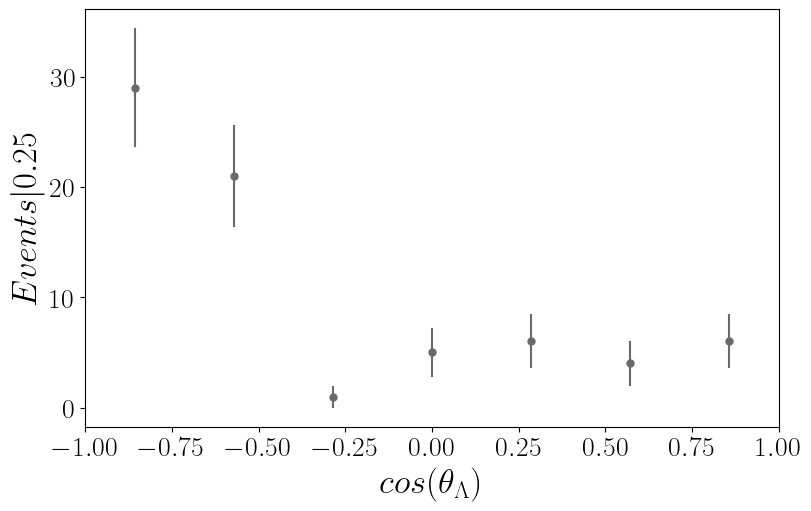
\includegraphics[width=1\columnwidth]{img/cos_theta_lambda.png}
    \end{minipage}
    \begin{minipage}[b]{0.5\columnwidth}
        \centering
        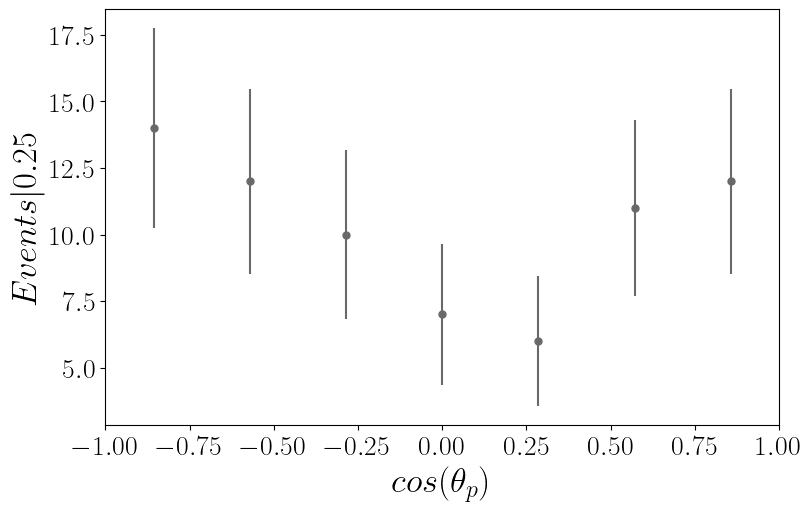
\includegraphics[width=1\columnwidth]{img/cos_theta_p.png}
    \end{minipage}
    
}

\begin{minipage}[b]{1\columnwidth}
    \centering
    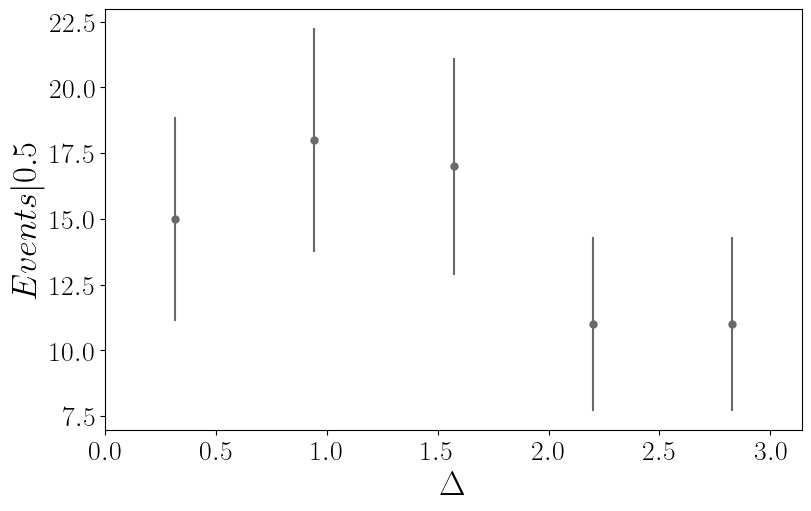
\includegraphics[width=0.5\columnwidth]{img/Delta.png}
\end{minipage}


\section{Выводы}
\tab На данный момент было затагировано всего $\sim 39000$ $\Lambda_c$, из которых согласно только 
бренченговому соотношению должно быть $\sim 503$ в канале $\Lambda_c \to \Lambda \pi$. 
Но после полной реконструкции события остается всего $77$. 
Для этих событий были получены распределения величин $\cos{\theta_\Lambda}, \ \cos{\theta_p}, \ \Delta$.

\tab Был предложен метод измерения формфакторов распада опираясь на связь со 
спиральными амплитудами и распределений углов, а так же метод улучшения опираясь 
на события $\Lambda_c \to \Lambda l \nu_l$ с известной спиральностью $W$-бозона.
\end{multicols}
\end{mdframed}

\begin{mdframed}[style=MyFrame]

\begin{enumerate}
    \item Abashian A., et al. The Belle Detector // Nuclear Instruments and Methods in Physics Research A. 2002. V. 479. P. 117–232.
    \item Eisenstein B. I., Alexander J. P., Berkelman K. Study of the Semileptonic Decay $\Lambda_c \rightarrow \Lambda e \nu_e$ // Physical Review D. 2022. V. 105. P. 012007. DOI: 10.1103/PhysRevD.105.012007.
    \item Richman J. D. An Experimenter’s Guide to the Helicity Formalism // J. D. Richman // CALT-68-1148.
    \item Bahtiyar H., Can K. U., Oka M., Takahashi T. T. $\Lambda_c \to \Lambda$ Form Factors in Lattice QCD // Phys. Rev. D. 2021. V. 102. P. 114505. DOI: 10.1103/PhysRevD.102.114505.    
\end{enumerate}

\end{mdframed}

\end{document}
